\chapter{Roadmaps in Continuous Spaces}
\label{chap:graphs-in-continuous}

Sweet, sweet chapter about how to best embed explicit graphs
in continuous configuration spaces.

In this chapter,
we'll primarly focus on single-query things,
but we'll keep in mind that we want things that can enable reuse eventually.

You get a bunch of benefit by patching
(you can apply LPA* efficiencly in outwards order).

By using graphs (and caching of structure)
we can completely eliminate nearest-neighbor queries!
Numbered graphs!

\section{Review of Alternative Approaches}
\label{sec:related-work}

Since $C$ is continuous,
all approaches must introduce some sort of discretization
in order to compute solutions.
We choose to build a graph consisting of vertices and edges in $C$,
and then search that graph (Section~\ref{sec:best-first}).
We do this because we can rely on existing techniques,
and because an explicit graph can be more easily reused than other
approaches.
In this section, we discuss alternative approaches to solving
the motion planning problem for articulated robots.

\subsection{Multi-Query Approaches}

We could run a PRM \cite{kavrakietal1996prm}.
Commit to a fixed graph,
and determine the validity of each vertex and edge w.r.t.
$\mathcal{C}_{\mbox{\scriptsize free}}$.
Then, at query time,
run A* to find the shortest path (this is fast due to graph sparseness).
This is good because it reuses work.
Unfortunately,
(a) our $\mathcal{C}_{\mbox{\scriptsize free}}$
is different for every subplan
(and for different options with each),
and (b) we don't want to determine validity over the entire graph
because it's costly.

\subsection{Anytime algorithms}

Compare to RRT*, FMT*, BIT*, etc.

\subsection{Other}

Need to look into the SBL planner \cite{sanchezante2001sbl}
(Single Query BiDirectional Lazy PRM).

\subsection{Incremental Construction Algorithms}

We could construct the graph incrementally and in response to the shape
of $\mathcal{C}_{\mbox{\scriptsize free}}$.
RRTs behave well for quickly finding feasible paths.
We'll compare against them at the end of this chapter.
Also talk about ESTs.
Difficult to cache things.

\subsection{Trajectory Optimization}

One approach is trajectory optimization.
For example, there's CHOMP \cite{zucker2013chomp}
and TrajOpt \cite{schulman2013trajopt}.
Lots of other prior work here that is not manipulation-focused.

Local minima problems.
Difficult to cache / apply to similar problems.

This is largely complementary.
Use sampling-based planning to quickly find feasible solutions,
and then optimize them.

\section{Building Graphs in Continuous Spaces}

\begin{itemize}
\item Probabalistic vs lattice-based graphs.
\item Probabalistic (pseudo-random) for efficient caching.
\end{itemize}

\section{Optimization in Expectation}

Extend the E$^8$-PRM algorithm to do things in expectation.

Relate to Evan's work.

Motivate the incremental densification idea,
with a graduated cost model
to approximate a probabalistic model
of the $\mathcal{C}$-space.

\section{Batching}

Choosing Batch Size $N$.
See Algorithm~\ref{alg:batched-e8}.

\begin{algorithm}
\caption{Batched-E$^8$ Planner}
\label{alg:batched-e8}
\begin{algorithmic}[1]
\Procedure {Batched-E$^8$}{$G, \mathcal{Q}, N, \lambda$}
%\State $G.V \leftarrow \emptyset$
%\State $G.E \leftarrow \emptyset$
\Loop
   \State \textsc{PrmAddSamples}($G, \mathcal{Q}, N$)
   \State Run E$^8$ ...
\EndLoop
\EndProcedure
\end{algorithmic}
\end{algorithm}

\begin{algorithm}
\caption{Partial Path Evaluation}
\label{alg:path-evaluation}
\begin{algorithmic}[1]
\Function {\textsc{EvalPath}}{$\pi$}
   \ForAll {$e \in \pi$}
         \label{line:edge-evaluation-order}
      \State $(S_{plan}, b_{plan}, c_{plan})
         = \mbox{\textsc{OptEdgePlan}}(e)$
      \ForAll {$X \in S_{plan}$}
         \State $b_{act} = \mathbf{1}_X[e]$
         \State $\arraycolsep=2pt
            e.P \leftarrow e.P \cup
            \left\{\left( \begin{array}{rl}
            \mathbf{1}_X & \mbox{if } b_{act} \\
            \lnot \mathbf{1}_X & \mbox{otherwise} \\
            \end{array} \right)
            \right\}$
         \If {$b_{act} \neq b_{plan}(X)$}
            \State \Return False
         \EndIf
      \EndFor
   \EndFor
   \State \Return True
\EndFunction
\end{algorithmic}
\end{algorithm}

The E$^8$-PRM (Algorithm~\ref{alg:e8})
operates on an initially empty persistent roadmap graph $G$.
Each vertex represents a configuration $x \in \mathcal{C}$,
and each edge represents a path $x(t)$ planned by a local planner.
Similarly to the LazyPRM,
edges are not evaluated until necessary.

The E$^8$-PRM proceeds in \emph{batches};
at the start of each batch,
the \textsc{PrmAddSamples} procedure adds
$N$ additional vertices to the graph sampled from $\mathcal{C}$
(including sampled start and goal configurations from $\mathcal{Q}$
if not yet present),
and edges are generated according to the PRM construction method.
The E$^8$-PRM does not commit to any particular such method
(e.g. r-disk, K-nearest-neighbors).

What graph are we searching over?
If it's too sparse, we'll stop after knowing that no solution exists.
If it's too dense, we'll spend too much time filling in parts of
space.
There's actually some spatial relationship in
$\mathcal{C}_{\mbox{\scriptsize free}}$ what we're not
modeling.
We get around this with artificial sparseness.
There's definitely a paper's worth of work here too (Shushman's stuff).
The easy version is with sequential batches of size $N$.
Talk about how what we really want to do
is evaluate the estimate of cost remaining
\emph{in expectation}.

Talk about how this is complementary to BIT* which acheive speedups
by batching, not by inflating.

Relate to Markov Random Fields and two-class image segmentation
which capture spatial correlation.

\section{Whole-Path Bisection Testing}

We implement the indicator functionals $\mathbf{1}_X[x(t)]$
approximately by evaluating the corresponding indicator functions
$\mathbf{1}_X(x)$ at a fixed resolution along the path.

Also talk here about the fancy Lazy PRM path bisection
evaluation function.

\section{The E$^8$-PRM}

This is the planner in continuous spaces,
requires a planning cost model for each edge.

\subsection{Implementation Details}
\label{subsec:implementation-details}

We provide an implementation of the E$^8$-PRM
as a plugin for the Open Motion Planning Library \cite{sucan2012ompl}.%
\footnote{Not available during the anonymous review process.}
Here, we discuss a few relevant details of the implementation.

\section{Execution Cost Models}

\begin{table}
   \centering
   \begin{tabular}{lc}
      \toprule
      Model & Additive? \\
      \midrule
      Path Length & Yes \\
      Bounded-Vel-Acc & Yes \\
      Smoothed & No \\
      \bottomrule
   \end{tabular}
   \caption{Execution cost models.
      Additive models admit efficient graph search methods
      when choosing optimistic paths for evaluation.}
   \label{table:exec-cost-models}
\end{table}

See Table~\ref{table:exec-cost-models}.

Could we relax the additive execution cost constraint?
We lose the nice efficient LPA*-enabling structure in
E$^8$ this way,
but it lets us incorporate a more accurate cost model in some domains,
especially for execution costs for fast motions (e.g. total time).

Sidd wants me to play with Hauser's fast bounded-velocity,
bounded-acceleration segment timing code
(which starts and stops at each waypoint).
This may have better performance,
choosing longer paths with few long edges over
shorter paths with many short edges.

\section{Future Work}

How to handle the narrow passage problem?
Lots of literature on that, new sampling strategies, etc.
(Toggle PRM, for instance.)

\section{Results}

I hope to show that the E$^8$-PRM is competitive with RRT-Connect
in terms of planning effort required to find a feasible path.

\begin{figure}
   \centering
   \begin{subfigure}[b]{0.3\textwidth}
      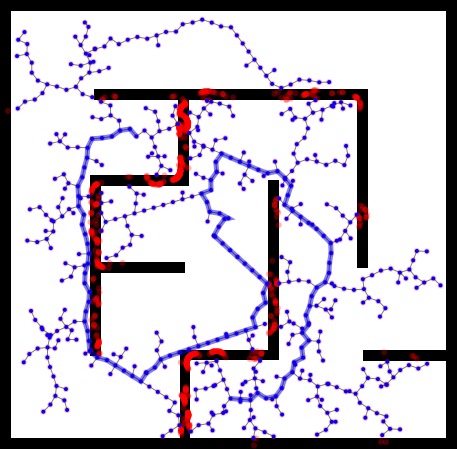
\includegraphics[width=\textwidth]{figs/compare-2d-rrtc1-rrtextcon-r1-s1.png}
      \caption{RRT Ext-Con, R=1}
   \end{subfigure}%
   \quad
   \begin{subfigure}[b]{0.3\textwidth}
      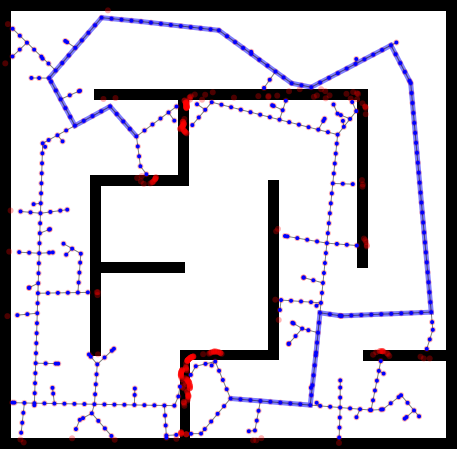
\includegraphics[width=\textwidth]{figs/compare-2d-rrtc1-rrtconcon-r1-s1.png}
      \caption{RRT Con-Con, R=1}
   \end{subfigure}%
   \quad
   \begin{subfigure}[b]{0.3\textwidth}
      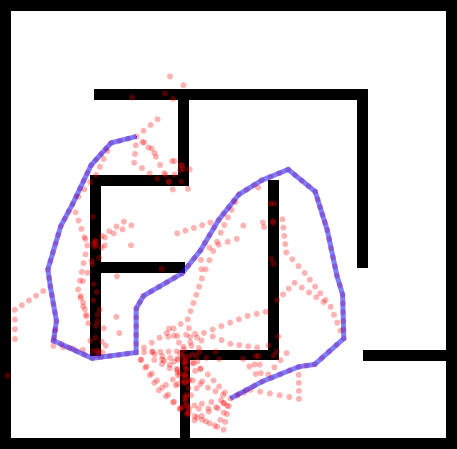
\includegraphics[width=\textwidth]{figs/compare-2d-rrtc1-checkmask-l00-s1.png}
      \caption{E$^8$-PRM, $\lambda=0$}
   \end{subfigure}%
   \vspace{0.05in}
   \begin{subfigure}[b]{0.3\textwidth}
      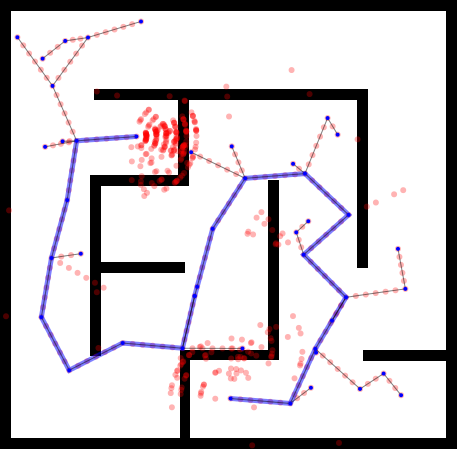
\includegraphics[width=\textwidth]{figs/compare-2d-rrtc1-rrtextcon-r6-s1.png}
      \caption{RRT Ext-Con, R=6}
   \end{subfigure}%
   \quad
   \begin{subfigure}[b]{0.3\textwidth}
      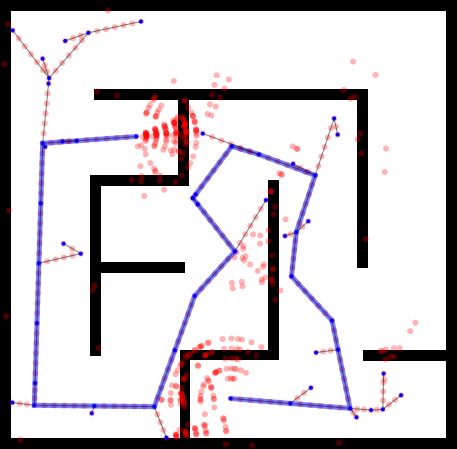
\includegraphics[width=\textwidth]{figs/compare-2d-rrtc1-rrtconcon-r6-s1.png}
      \caption{RRT Con-Con, R=6}
   \end{subfigure}%
   \quad
   \begin{subfigure}[b]{0.3\textwidth}
      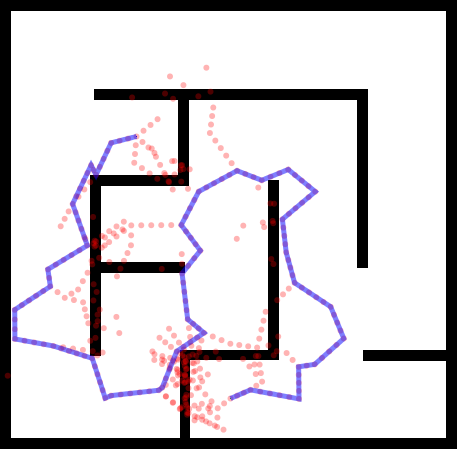
\includegraphics[width=\textwidth]{figs/compare-2d-rrtc1-checkmask-l10-s1.png}
      \caption{E$^8$-PRM, $\lambda=1$}
   \end{subfigure}%
   \caption{Example runs with different planners,
      with the same sequence of samples.
      Note that E$^8$-PRM with $\lambda=0$ is equivalent to LazyPRM.
      Red dots show collision checks.}
   \label{fig:compare-2d-rrtc1-vis}
\end{figure}

\begin{figure}
\centering
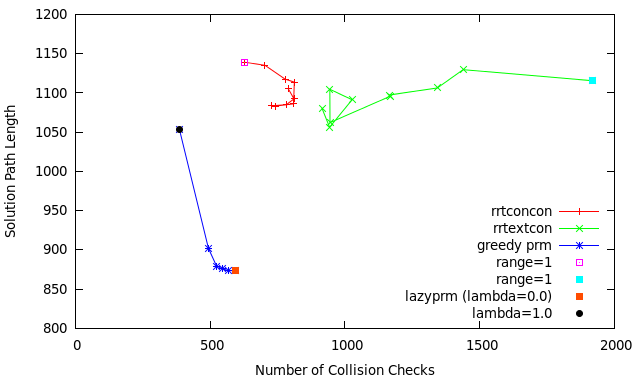
\includegraphics[width=0.8\textwidth]{figs/compare-2d-rrtc1-medians.png}
\caption{Plot of collision checks vs solution path cost for the
   different algorithms from the problem from
   Figure~\ref{fig:compare-2d-rrtc1-vis}.}
\end{figure}

\begin{figure}
   \centering
   \begin{subfigure}[b]{0.4\textwidth}
      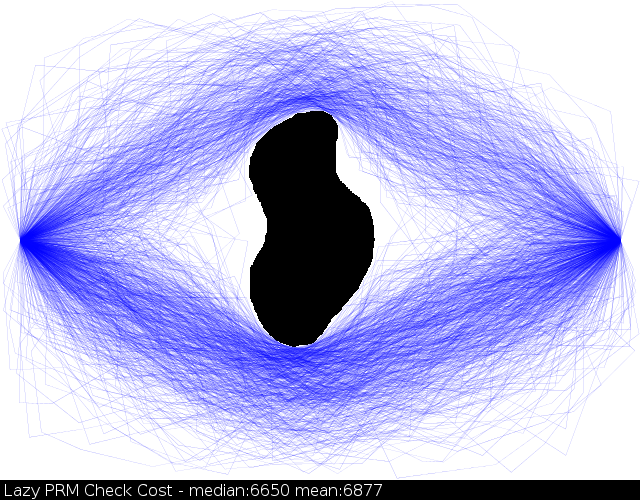
\includegraphics[width=\textwidth]{figs/timegreedy-bean-lambda-00.png}
      \caption{Paths with $\lambda = 0$}
   \end{subfigure}%
   \quad
   \begin{subfigure}[b]{0.4\textwidth}
      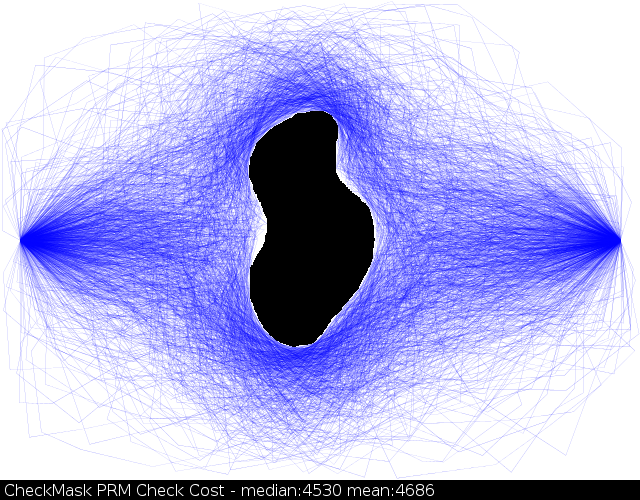
\includegraphics[width=\textwidth]{figs/timegreedy-bean-lambda-10.png}
      \caption{Paths with $\lambda = 1$}
   \end{subfigure}%
   \caption{Examples of paths for a 2d problems
      for different values of $\lambda$.
      As $\lambda$ is increased,
      paths are longer, but are faster to find.}
   \label{fig:bean}
\end{figure}

\begin{figure}
   \centering
   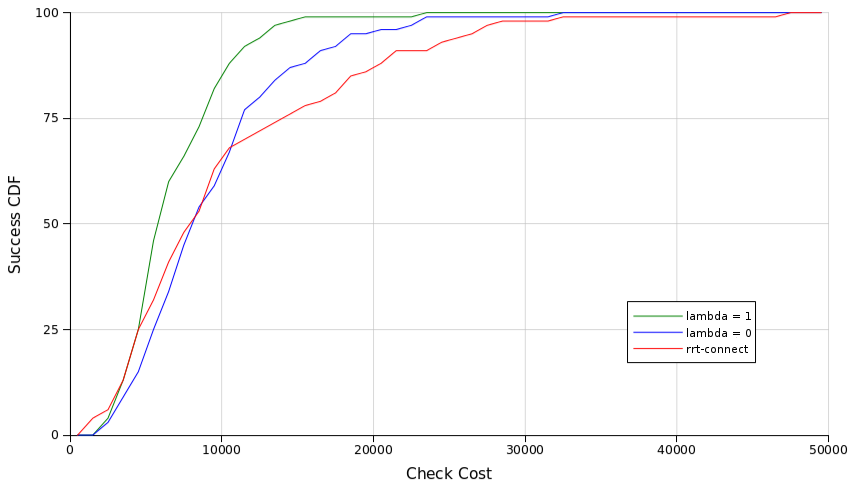
\includegraphics[width=0.8\textwidth]{figs/timegreedy-herbstep1-comparison-cdfs.png}
   \caption{Comparison between different algorithms on a HERB problem.
      Must add in ESTs.}
   \label{fig:herb-comparison-cdfs}
\end{figure}

